\documentclass[12pt]{article}

\usepackage{import}
\usepackage{standalone}

\usepackage[top=4cm, right=2cm, bottom=2.7cm, left=2cm]{geometry}

\usepackage{wrapfig}
\usepackage{tabulary}
\usepackage{float}
\usepackage{pifont}
\usepackage{background}
\usepackage{tikz}


\pagestyle{empty}
\setlength{\parindent}{0pt}

\begin{document}
	\begin{minipage}{\textwidth}
		\section{Animatie \hfill\small Bron: Bebras}
		Alice wil graag haar website opvrolijken met een animatie van een rijdende auto. Daarvoor heeft ze vier afbeeldingen gemaakt.
		
		In welke volgorde moet je de afbeeldingen tonen om de indruk te wekken dat de auto zich naar rechts verplaatst? 
		
		\begin{table}[H]
			\begin{tabulary}{\linewidth}{|C|CCCC|}
				\hline 
				\textbf{A} & 
				\vspace{0.01cm}
\includegraphics[width=\linewidth]{option1} &
				\vspace{0.01cm}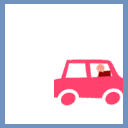
\includegraphics[width=\linewidth]{option4} &
				\vspace{0.01cm}
\includegraphics[width=\linewidth]{option2} &
				\vspace{0.01cm}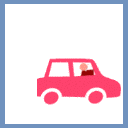
\includegraphics[width=\linewidth]{option3}
				\\ \hline 
				\textbf{B} &
				\vspace{0.01cm}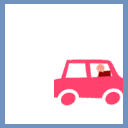
\includegraphics[width=\linewidth]{option4} &
				\vspace{0.01cm}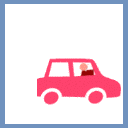
\includegraphics[width=\linewidth]{option3} &
				\vspace{0.01cm}
\includegraphics[width=\linewidth]{option2} &
				\vspace{0.01cm}
\includegraphics[width=\linewidth]{option1}
				\\ \hline
				\textbf{C} &
				\vspace{0.01cm}
\includegraphics[width=\linewidth]{option1} &
				\vspace{0.01cm}
\includegraphics[width=\linewidth]{option2} &
				\vspace{0.01cm}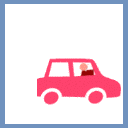
\includegraphics[width=\linewidth]{option3} &
				\vspace{0.01cm}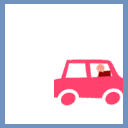
\includegraphics[width=\linewidth]{option4}
				\\ \hline
				\textbf{D} &
				\vspace{0.01cm}
\includegraphics[width=\linewidth]{option1} &
				\vspace{0.01cm}
\includegraphics[width=\linewidth]{option1} &
				\vspace{0.01cm}
\includegraphics[width=\linewidth]{option1} &
				\vspace{0.01cm}
\includegraphics[width=\linewidth]{option1}
				\\ \hline
			\end{tabulary}
		\end{table}
	\end{minipage} \\ \\
	
\end{document}